\chapter{\He Tubes}
\label{chap:he3tube}

\section{Description}


\begin{figure}[htb]
	\centerfloat
		\includegraphics[scale=0.25]{images/he3tubePhoto}
	\caption[\He tube]{\He tube (see Fig~\ref{fig:he3spec} for a detailed schematic of the detector).}
	\label{fig:he3photo}
\end{figure}

	Four \he tubes were procured from GE-Reuter Stokes for the purpose of thermal neutron detection in BEAST~II. They consist of stainless steel tubes 9.47$^{\verb+"+}$ long and 2$^{\verb+"+}$ in diameter filled with $^3$He at 4 atm of pressure. 


\section{Theory of Operation}

When a thermal neutron (with an energy of 0.025 eV) passes through the active area of the detector, it may be captured by a $^3$He atom~\cite{Oed200462}:

\begin{equation}
		{^{3}_{2}\mathrm{He}+^{1}_{0}\mathrm{n}\rightarrow~^{3}_{1}\mathrm{H}+^{1}_{1}H+764~\mathrm{keV}}
\end{equation}

The cross section for this reaction decreases as the energy of the neutron increases, as shown in Fig~\ref{fig:neutCross}. The $^3$H and proton ionize the gas in the tubes. This ionization produces a signal on a sense wire in the centre of the tube.

	The signal is read out by a custom amplifier system designed and built by the electronics shop at the University of Victoria. 


\begin{figure}[htb]
	\centerfloat
		\includegraphics[width=\textwidth]{images/neutron_cross_section}
	\caption[Cross section of neutron capture by \he as a function of neutron energy]{Cross section of neutron capture by \he as a function of neutron energy. The vertical black line corresponds to upper range of the energy of thermal neutrons~\cite{BNL}.}
	\label{fig:neutCross}
\end{figure}


\section{Readout Electronics}

	The \he tube amplification system consists of two devices: an amplifier module that is attached directly to the back end of the tube (see Figs~\ref{fig:he3ampfront} and~\ref{fig:he3ampread}), and a receiver box that plugs into a slot in a NIM crate (see Fig~\ref{fig:he3Rec}). Both of these devices were designed and built in the electronics shop in the physics department at the University of Victoria.

\begin{figure}[htb]
    \centering
    \begin{tabular}{ccc}
	\subfigure[Amplifier Front]{\includegraphics[scale=0.12]{images/preampPhoto}\label{fig:he3ampfront}} & 
	\multirow{-3}[18]{*}{\subfigure[Receiver box]{\includegraphics[height=6.2cm]{images/RecieverBoxPhoto}\label{fig:he3Rec}}} &
	\multirow{-3}[18]{*}{\subfigure[Power supply]{\includegraphics[height=6.2cm]{images/bertan}\label{fig:he3HV}}} \\
	\subfigure[Amplifier Rear]{\includegraphics[scale=0.12]{images/preampPhoto2}\label{fig:he3ampread}}\\
    \end{tabular}
    \caption[Amplifier module, receiver box, and power supply]{Amplifier module, receiver box, and power supply. Circuit diagrams can be found in Appendix~\ref{chap:he3spec}.}
    \label{fig:he3ampRec}
\end{figure}


\subsection{Amplifier Module}

	The amplifier module is attached to the end of the \he tube. It is connected to the sense wire of the \he tube via a 47~pF capacitor to remove the high voltage (HV) on the sense wire. This amplifier provides a gain of 2. Once the signal is amplified, it is sent through a differential line driver. The signal is split into two identical components, one of which has its polarity reversed. These signals are then sent down a twisted pair CAT-6 cable. Low voltage power for the amplifier circuitry is also provided by the CAT-6 cable. A circuit diagram can be z~\ref{fig:he3preampLineDriver}~\cite{Honkanen}.

	In addition to amplifying the \he tube signal, the amplifier module also routes high voltage of 1.58~kV to the sense wire in the tube. This high voltage is produced by a Bertan model 323 HV power supply (see Fig~\ref{fig:he3HV}).


\subsection{Receiver Box}

	The receiver box contains integrated circuits (ICs) which receive the signal from the CAT-6 cable, and provides the low voltage to power the amplifier circuit in the amplifier modules. The split signal from the amplifier is combined at the receiver box. This differential signal approach should reduce most electronic noise, since the noise should affect both the inverted signal and the non-inverted signals and any noise which affects both will be removed when the two are combined. The receiver box outputs the signals via lemo connections on the front. The box contains four separate ICs, and as such can handle the signals from four different tubes. It is powered by the NIM back plane. A circuit diagram can be found in Fig~\ref{fig:he3LineReciever}~\cite{Honkanen}.



\section{Data Acquisition}

	Data acquisition (DAQ) is performed with a CAEN 1724 digitizer (Fig~\ref{fig:CAENDIGI}). This device receives the signals from the receiver box and records the pulse height and time of a signal waveform, with a time resolution of 20 ns. This information is then passed to a computer via a VME-USB bridge (Fig~\ref{fig:CAENCON}).


\begin{figure}[htb]
    \centering
    \begin{tabular}{cc}
	\subfigure[V1724 Digitizer]{\includegraphics[height=3in]{images/V1724}\label{fig:CAENDIGI}}&
	\subfigure[V1718 Controller]{\includegraphics[height=3in]{images/Controller}\label{fig:CAENCON}} \\
    \end{tabular}
    \caption[CAEN VME modules used for DAQ]{CAEN VME modules used for DAQ.}% Specifications can be found in Table~\ref{tab:CAENSPEC}}
    \label{fig:VMEmod}
\end{figure}


	DAQ software was written to combine the CAEN digitizer libraries, the \textbf{E}xperimental \textbf{P}hysics and \textbf{I}ndustrial \textbf{C}ontrol \textbf{S}ystem (EPICS) \cite{EPICS}, and the ROOT data analysis framework \cite{CERNROOT}. EPICS is used for slow control of all BEAST~II subsystems and to get real time plots of the data as the experiment is running. In the case of the \he tubes, EPICS controls starting and stopping of acquisition and reports the rate of hits in the \he tubes to the operator. ROOT ntuples containing the channel number, pulse height, and time stamp (in seconds since January 1, 1970) are saved to disc by the DAQ software.


	The digitizer has a 21~s (30 bit counter, 20~ns/bit) clock on board which is used to set the time stamp. After 21~s, this internal clock resets to 0 which the CAEN software accounts for on the next trigger. Unfortunately, when the clock rolls over multiple times without a trigger, the CAEN software assumes the clock has only rolled over once, leading to an incorrect time stamp. To prevent this, EPICS sends a software trigger to the digitizer every 10~s to ensure that the clock never rolls over more than once between triggers. This 0.1~Hz software trigger rate is subtracted from the \he tube hit rate in the analysis.



\section{Calibration}

After Phase~I was complete, the \he tubes were shipped back to the University of Victoria for calibration. This was a calibration of the whole system: the tubes themselves, the preamplifiers, the digitizer, and GEANT4 (v10.3). During the calibrations, each tube was connected to the same channel that it was during Phase~I.

\subsection{Neutron Source}
\label{sec:AmBe}
	The University of Victoria has a 241-AmBe neutron source, which produces neutrons using the following reaction \cite{barschall1983neutron}:

\begin{subequations}
\begin{align}
		{^{241}_{95}\mathrm{Am}\rightarrow~^{237}_{93}\mathrm{Np} + ^4_2\mathrm{He} + \gamma}\\
		{^9_4\mathrm{Be}+^4_2\mathrm{He}\rightarrow~^{12}_6\mathrm{C}+^1_0\mathrm{n}+\gamma}
\end{align}
\end{subequations}
with an activity of 168~GBq (measured at 185~GBq in 1966). The energy spectrum of an AmBe source can be found in Fig~\ref{fig:AmBeSpec}. The configuration of the University of Victoria's AmBe source can be found in~\cite{hargrove}. The neutron rates from five different AmBe sources is measured in \cite{lebreton2007experimental}. From this, it is determined that an AmBe source produces 6.08$\pm$0.17$\times10^{4}$~neutrons/GBq. For the 168~GBq source, this corresponds to 1.02$\pm$0.03$\times10^{7}$~neutrons/s.

The source is surrounded by a cube of graphite 1.83~m to a side, which thermalizes the neutrons. The spectrum of the neutrons which emerge from the graphite is shown in Fig~\ref{fig:afterGraphite}. For reference, the efficiency of the \he tubes over a large kinetic energy range is shown in Fig~\ref{fig:he3eff}. Using data from these figures, the \he tubes are able to detect 62\% of the neutrons which emerge from the graphite cube. Graphite can contain boron impurities, but since the graphite used next to the source is `medium grade' it is assumed that there is no significant absorption of neutrons by boron impurities. This graphite has a density of (1.63$\pm$0.01)~g/cm$^3$~\cite{AmBELetter}. This source provides an excellent tool for testing and calibrating the \he tubes. 

\begin{figure}
	\centerfloat
		\includegraphics[trim={0 0 0 0.75cm},clip, width=\textwidth]{images/AmBe_NeutronSpectrum.pdf}
	\caption[Energy spectrum of neutrons from AmBe source]{Energy spectrum of neutrons from AmBe source~\cite{AmBeSpec}.}
	\label{fig:AmBeSpec}
\end{figure}


\begin{figure}
	\centerfloat
		\includegraphics[trim={0 0 0 0.75cm},clip, width=\textwidth]{images/AfterGraphite}
	\caption[Kinetic energy spectrum of neutrons after they pass through the graphite cube]{Kinetic energy spectrum of neutrons after they pass through the graphite cube. From simulation in GEANT4.}	
	\label{fig:afterGraphite}
\end{figure}


\begin{figure}
	\centerfloat
		\includegraphics[trim={0 0 0 0.75cm},clip, width=\textwidth]{images/Efficiency_inside}
	\caption[Efficiency of \he tubes vs kinetic energy]{Efficiency of \he tubes vs kinetic energy, from simulation in GEANT4.}
	\label{fig:he3eff}
\end{figure}


\subsection{Calibration Procedure}


\subsubsection{Gain Matching}

	The \he tubes were returned to the University of Victoria after Phase~I of BEAST~II operation for calibration. During testing, it was observed that the pulse height spectrum for each \he tube did not match the pulse height spectrum from the same tube in Phase~I, despite having the HV supply set to the same voltage (see Fig~\ref{fig:pulseHeightSpectrumDifferenceBaA}). It is unclear what caused this issue, but subsequent measurements of the output voltage of the Bertran supply suggests that it was not as stable as expected. In order to get an accurate calibration, it was necessary to choose an HV setting that caused the pulse height spectrum to match what was observed in Phase~I. 

	The \he tubes were run at 2~V increments starting from 1540~V up to 1590~V. For each voltage setting, $\chi^2$ comparison was done between the spectrum observed in Phase~I and the spectrum observed at that voltage. The voltage that produced the lowest $\chi^2$ was used as the operating voltage for that tube during calibration. Table~\ref{tab:Tubevoltage} summarizes the voltage settings used in Phase~I. 


\begin{figure}
	\centering
	\subfigure[Channel 0]{
		\begin{overpic}[trim={0 0 0 0.5cm},clip, width=0.47\textwidth]{images/VoltageTestChannel0.pdf}
		\end{overpic}
		\label{fig:VoltageChannel0}
	}
	\subfigure[Channel 1]{
		\begin{overpic}[trim={0 0 0 0.5cm},clip, width=0.47\textwidth]{images/VoltageTestChannel1.pdf}
		\end{overpic}
		\label{fig:VoltageChannel1}
	}
	\subfigure[Channel 2]{
		\begin{overpic}[trim={0 0 0 0.5cm},clip, width=0.47\textwidth]{images/VoltageTestChannel2.pdf}
		\end{overpic}
		\label{fig:VoltageChannel2}
	}
	\subfigure[Channel 3]{
		\begin{overpic}[trim={0 0 0 0.5cm},clip, width=0.47\textwidth]{images/VoltageTestChannel3.pdf}
		\end{overpic}
		\label{fig:VoltageChannel3}
	}
	\caption[Pulse height spectra before and after voltage correction]{Pulse height spectra of thermal neutrons before and after voltage correction. Red is during Phase~I, blue is at 1580 V, and green is at the corrected voltage.}
	\label{fig:pulseHeightSpectrumDifferenceBaA}
\end{figure}




\paragraph{Uncertainty on the rate due to the voltage setting} Since the voltage that was used to calibrate the \he tubes is not exactly the same as the voltage used in Phase~I, there is an uncertainty in the calibrated rate. To quantify this uncertainty, the rate at the chosen voltage setting was compared to the rates measured at +2~V and -2~V, since these were the smallest voltage increments studied and serve as a conservative uncertainty. The uncertainty due to the voltage setting is then:
\begin{equation}
	{\sigma_{\pm} = |R_{\mathrm{nominal}} - R_{\mathrm{nominal}\pm2\mathrm{ V}}| }
\end{equation}
The values of $\sigma_{\pm}$ are presented in Table~\ref{tab:VoltageUncertainty}.





\begin{table}[htb]
	\centering
	\begin{tabular}{ cc }
	Channel	& Voltage (V)	\\ \hline \hline
	0	& 1586	\\
	1	& 1570	\\
	2	& 1550	\\
	3	& 1560	\\ \hline
	\end{tabular}
	\caption[Nominal high voltage settings during \he tube calibration]{Nominal high voltage settings during \he tube calibration.}
	\label{tab:Tubevoltage}
\end{table}


\begin{table}[htb]
	\centering
	\begin{tabular}{ cccccc }
	&	\multicolumn{3}{c}{Rate at} & & \\
Channel	&	-2~V (Hz)	&	Nominal (Hz)	&	+2~V (Hz)	&	$\sigma_+$ (Hz)	&	$\sigma_{-}$ (Hz)	\\ \hline
0	&	199.0	&	191.6	&	184.8	&	7.47	&	6.75	\\
1	&	218.4	&	214.2	&	198.0	&	4.20	&	16.24	\\
2	&	140.3	&	146.2	&	158.5	&	12.35	&	5.93	\\
3	&	255.8	&	262.1	&	271.8	&	6.38	&	9.64	\\ \hline
	\end{tabular}
	\caption[Uncertainty on \he tube rate due to voltage uncertainty]{Uncertainty on \he tube rate due to voltage uncertainty.}
	\label{tab:VoltageUncertainty}
\end{table}





\subsection{Calibration}

To calibrate the \he tubes, each tube was placed one at a time into a cradle made of high density polyethylene (HDPE). The polyethylene reduced the thermal neutron flux in the source room from $\sim$600~Hz to $\sim$100~Hz, similar to that observed in Phase~I of BEAST~II, by absorbing some of the thermal neutrons. The relative orientation of the \he tubes and the graphite is shown in Fig~\ref{fig:he3CalibPosn}. 

\begin{figure}[htb]
	\centerfloat
	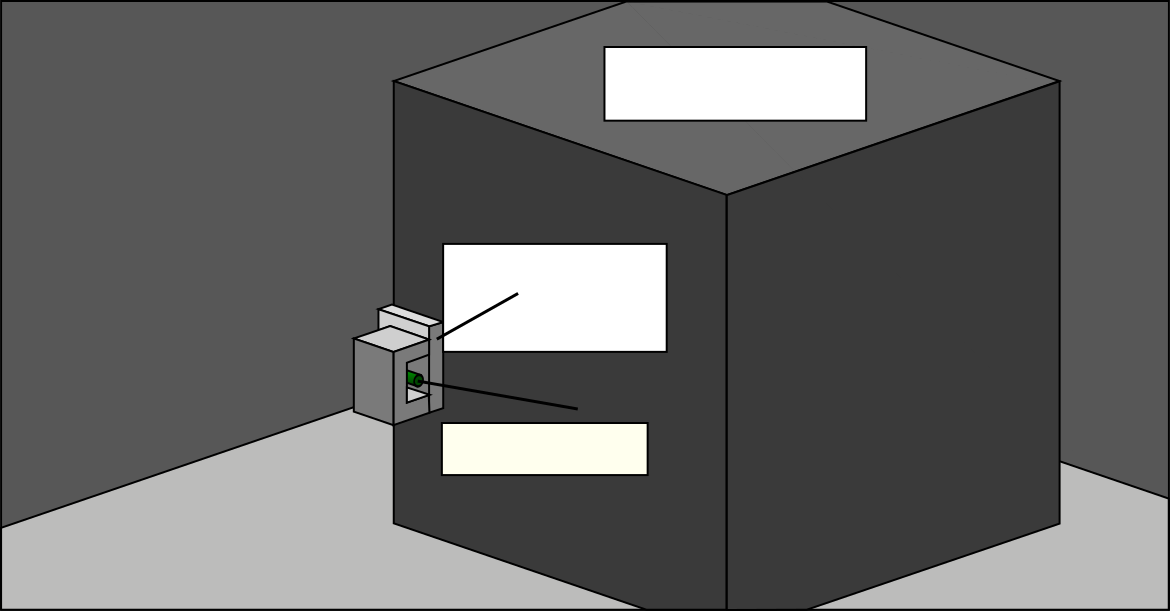
\includegraphics[height=8cm]{images/GEANTVis2}
	\caption[\He tube calibration setup]{\He tube calibration setup from GEANT4 simulation, including HDPE cradle. Image is to scale.}	
	\label{fig:he3CalibPosn}
\end{figure}



The rate in each \he tube was recorded, then the cradle was moved to a position further from the source and the process was repeated. The rate in each \he tube as a function of the distance from the source is given in Fig~\ref{fig:he3rateVsD}.



\subsubsection{AmBe Source Simulation}
\label{sec:ambesim}

	A simulation of the AmBe source was produced using GEANT4 \cite{GEANT}. The simulation contains the source, the graphite cube (using the GEANT4 default density of 1.7~g/cm$^3$ instead of 1.63~g/cm$^3$), the concrete walls of the room, the HDPE cradle, and the \he tube. Neutrons following the spectrum shown in Fig~\ref{fig:AmBeSpec} are fired isotropically from the centre of the graphite cube. 1.0$\times10^{7}$ events corresponds to 1 second.


\begin{figure}
	\centerfloat
		\includegraphics[trim={0 0 0 0.75cm},clip, width=\textwidth]{images/Parallel_Calibration}
	\caption[\He tube rate vs distance from thermal neutron source]{\He tube rate vs distance from thermal neutron source. Orange is simulation, other colours are the different channels. The measured minus fit rates are presented in Fig~\ref{fig:he3rateVsDUncertainty}.}	
	\label{fig:he3rateVsD}
\end{figure}

\begin{figure}
	\centerfloat
		\includegraphics[width=\textwidth]{images/Parallel_Calib_Uncertainties}
	\caption[\He tube rate minus fit vs distance from thermal neutron source]{\He tube rate minus fit vs distance from thermal neutron source. Orange is simulation, other colours are the different channels. The errors are statistical only.}	
	\label{fig:he3rateVsDUncertainty}
\end{figure}


\subsubsection{Curve Fitting}

	The rates are fit to an inverse square function:
\begin{equation}
	{R_{n} = A_{n}\times\left(\frac{B}{(r-r_{0})^2}+C\right)}
	\label{eqn:invSq}
\end{equation}	
where $r$ is the position of the \he tube relative to the AmBe source. The parameters $B$, $C$, and $r_{0}$ are shared by the four \he tubes, while $A_{n}$ varies in each \he tube.

The AmBe source room is significantly more complex than just a graphite cube with a source at its centre as there is a large amount of equipment and storage in the room. This extra material is very difficult to simulate, but should manifest as a background neutron rate in the room, and thus only affect the `C' term in the fit. Therefore, a modified version of Eqn~\ref{eqn:invSq} is used for the simulation:
\begin{equation}
	{R_{\mathrm{sim}} = A_{\mathrm{sim}}\times\left(\frac{B}{(r-r_{0})^2} + C\right)+C_{\mathrm{sim}}}
\end{equation}	
The parameters $B$, $C$, and $r_0$ are the same as used in the fit to data. The fit to data and simulation are done simultaneously, with $A_{\mathrm{sim}}$ fixed at 1. $A_{n}$ is therefore the efficiency of each tube relative to the simulation. The efficiency for each \he tube is presented in Table~\ref{tab:he3Calib}.  The other fit parameters can be found in Table~\ref{tab:CalibrationFitPars}. The uncertainty due to the voltage setting is calculated as:
\begin{equation}
	{\sigma_{\pm}^V = A_{n}\frac{\sigma_{\pm}}{R}}
\end{equation}
where $\sigma_{\pm}$ and $R$ are taken from Table~\ref{tab:VoltageUncertainty}. 

Additionally, a 3\% uncertainty is added to account for the uncertainty on the number of neutrons produced by the AmBe source (see \S~\ref{sec:AmBe}).

The uncertainties due to the voltage, the neutron production rate, and from the fit are combined in quadrature to get the total uncertainty.

The measured rate minus the fit rate is shown in Fig~\ref{fig:he3rateVsDUncertainty}.

\begin{table}[htb]
	\centering
	\begin{tabular}{ cccccccccc}
Channel	&	$A_{n}$	&	$\sigma^{\mathrm{fit}}$	&	$\sigma_{+}^{V}$	&	$\sigma_{-}^{V}$	&	$\sigma^{\mathrm{AmBe}}$&		$\sigma_{+}^{\mathrm{Tot}}$	&	$\sigma_{-}^{\mathrm{Tot}}$	\\	\hline	\hline
0	&	0.278	&	0.019	&	0.011	&	0.010	&	0.008	&	0.023	&	0.021	\\		
1	&	0.282	&	0.020	&	0.006	&	0.021	&	0.008	&	0.021	&	0.029	\\		
2	&	0.154	&	0.011	&	0.013	&	0.006	&	0.005	&	0.017	&	0.013	\\		
3	&	0.201	&	0.014	&	0.007	&	0.005	&	0.006	&	0.016	&	0.015	\\	\hline	
	


	\end{tabular}
	\caption[\He tube efficiency with uncertainties]{\He tube efficiency with uncertainties. $\sigma^{\mathrm{fit}}$ is the uncertainty from the fitting, $\sigma_{\pm}^{V}$ is the uncertainty from the voltage, and $\sigma^{\mathrm{AmBe}}$ is the uncertainty from the neutron production rate.}
	\label{tab:he3Calib}
\end{table}

\begin{table}[htb]
	\centering
	\begin{tabular}{ lrrr }
Parameter		& Value		& Uncertainty	 \\ \hline \hline
	$\chi^2$		& 215.361	& 		\\
	degrees of freedom		& 47		&		\\
	$B\times10^{6}$ cm$^2$s$^{-1}$ 	&	7.243 	& 0.822 	\\	
$	r_{0}$ (cm)	&	0 			& 4.6 	\\	
	$C$ (Hz)	&	107.856				& 10.2 	\\	
$	A_{0}	$	&	0.278				& 0.019	\\	
$	A_{1}	$	&	0.282				& 0.020	\\	
$	A_{2}	$	&	0.154				& 0.011	\\	
$	A_{3}	$	&	0.201				& 0.014	\\	
$	A_{\mathrm{sim}}	$	&	1.000				& N/A	\\	
$	C_{\mathrm{sim}}	$ (Hz)	&	100.455				& 26.4 	\\	\hline

	\end{tabular}
	\caption[Fit parameters for calibration fit shown in Fig~\ref{fig:he3rateVsD}]{Fit parameters for calibration fit shown in Fig~\ref{fig:he3rateVsD}.}
	\label{tab:CalibrationFitPars}
\end{table}

\paragraph{Uncertainty on points}

	The uncertainty on the simulated points is the square root of the number of simulated hits divided by number of seconds that have been simulated:
\begin{equation}
	\sigma_{\mathrm{rate}} = \frac{\sqrt{N_{\mathrm{events}}}}{t}
	\label{eqn:rateUncertainty}
\end{equation}

	The measured data have two associated uncertainties: the uncertainty on the rate, and the uncertainty on the position. The uncertainty on the rate is the same as also given by Eqn~\ref{eqn:rateUncertainty}. The uncertainty on the position is taken to be 1 cm. 

The position uncertainty is converted to a rate uncertainty using standard propagation of error:
\begin{equation}
	\sigma_{\mathrm{rate}}^{\mathrm{position}} = \frac{\partial R_{n}}{\partial r}\sigma_{r}= 2\frac{A_{n}B}{(r-r_0)^3}\sigma_{r}
	\label{eqn:posUncert}
\end{equation}
where $R_{n}$ is given by Eqn~\ref{eqn:invSq}.
Equations~\ref{eqn:rateUncertainty} and~\ref{eqn:posUncert} are added in quadrature to get the total rate uncertainty. Since the uncertainty due to the position requires fit parameters to calculate, the fit is first calculated, then the uncertainty on the rate due to position is calculated. The fit is then recalculated until the fit parameters converge. The uncertainty on the rate is shown in Fig~\ref{fig:he3rateVsDUncertainty}.

\paragraph{Discussion of $\chi^{2}$}

	As evident from Table~\ref{tab:CalibrationFitPars}, the $\chi^2$ of the calibration fit is quite high. Because the fit is done for all four tubes and simulation simultaneously, an outlying point in one of the tubes affects the whole calibration. In Fig~\ref{fig:he3rateVsD}, the first three points of channel 0 are outliers. These are the main contribution to the large $\chi^2$ value. If these first three points are removed and the fit is recalculated, $\chi^2$ becomes 110.4, with 44 degrees of freedom. A comparison of the efficiencies ($A_{n}$) and C$_{\mathrm{sim}}$ with and without these points can be found in Table~\ref{tab:he3ChiCompare}. The values of $A_{n}$ are consistent within 1 $\sigma$.

\begin{table}[htb]
	\centering
	\begin{tabular}{ccccc}
	&		&		&	 \multicolumn{2}{c}{Removing first three}			\\	
	&	 \multicolumn{2}{c}{All points}			&	 \multicolumn{2}{c}{points of channel 0}			\\	
Channel	&	$A_{n}$	&	$\sigma_{A_{n}}$	&	$A_{n}$	&	$\sigma_{A_{n}}$	\\ \hline \hline	
0	&	0.278	&	0.019	&	0.294	&	0.020	\\	
1	&	0.282	&	0.020	&	0.294	&	0.020	\\	
2	&	0.154	&	0.011	&	0.160	&	0.011	\\	
3	&	0.200	&	0.014	&	0.209	&	0.014	\\	
C$_{\mathrm{sim}}$ &  100.455 & 26.4    &	114.324 &	25.186  \\	\hline

	\end{tabular}
	\caption[\He tube efficiencies with and without first three channel 0 points]{\He tube efficiencies with and without first three channel 0 points.}
	\label{tab:he3ChiCompare}
\end{table}


\paragraph{Cross Check on \He Tube Efficiency}

	The uncertainty on the \he tube efficiency is the uncertainty on the fitting parameters shown in Table~\ref{tab:CalibrationFitPars}. As a cross check, a simple analysis was done.

	Each simulated point has the parameter $C_{\mathrm{sim}}$ subtracted from it. Then, for each data point, an estimate of $A$ was calculated:
\begin{equation}
	A_{\mathrm{Estimate}} = \frac{R_{\mathrm{real}}}{R_{\mathrm{sim}}-C_{\mathrm{sim}}}
\end{equation}
For each tube, the mean and RMS of this was calculated for all points in Fig~\ref{fig:he3rateVsD} (Table~\ref{tab:CrossCheck}). The RMS calculated in this cross check was very similar to the fit uncertainties shown in Table~\ref{tab:CalibrationFitPars}, which provides evidence that the fitting uncertainties are appropriate, even for large $\chi^2$.


\begin{table}[htb]
	\centering
	\begin{tabular}{ ccc }
Channel	&	$A_{\mathrm{Estimate}}$	&	RMS	\\ \hline \hline	
0	&	0.275	&	0.020	\\	
1	&	0.281	&	0.019	\\	
2	&	0.155	&	0.011	\\	
3	&	0.201	&	0.012	\\	\hline

	\end{tabular}
	\caption[Cross check of uncertainty on \he tube efficiency]{Cross check of uncertainty on \he tube efficiency.}
	\label{tab:CrossCheck}
\end{table}





	%To quantify the uncertainty on the \he tube efficiency, the maximum and minimum value of this equation was used:

%	Each simulated point had the parameter $C_{sim}$ subtracted from it. Then for each tube, the maximum and minimum of $R_{real}/R_{sim}$ are found. The uncertainty $\sigma_{\pm}^{fit}$ is then defined as:
%\begin{equation}
%\sigma_{\pm}^{fit} = |A_{n} - A_{n}^{\pm}|
%\end{equation}
%where $A_{n}^{+}$ is the maximum value of $R_{real}/R_{sim}$, and $A_{n}^{-}$ is the minimum.  The uncertainty from the fitting was combined with the uncertainty due to the voltage to get the total uncertainty. The uncertainties can be found in Table~\ref{tab:he3Calib}



%	To quantify the uncertainty on the \he tube efficiency, the fitting of the \he tube vs distance from the source was repeated, ignoring the first four data points, as these have the largest deviation from the fit shown in~\ref{fig:he3rateVsD}. The fit was then repeated ignoring the last six data points. The efficiencies produced by these fits provided an upper and lower bound on the values for the \he tube efficiency, and are used as uncertainty on the fit. Plots of these fits can be found in Appendix~\ref{chap:calibUn}. The uncertainty from the fitting was combined with the uncertainty due to the voltage to get the total uncertainty. The uncertainties can be found in Table~\ref{tab:he3Calib}.
	

	%The fit shown in Fig~\ref{fig:he3rateVsD} 


\section{Deployment in BEAST~II Phase~I}



\begin{figure}[htb]
	\centerfloat
		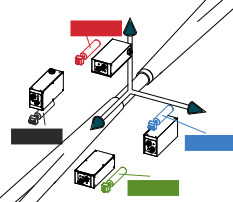
\includegraphics[width=\textwidth]{images/he3tubesAndTPCs}		
	\caption[\He tube and TPCs in BEAST~II Phase~I]{\He tube and TPCs in BEAST~II Phase~I. Colour scheme is the same as used in various plots, such as Fig~\ref{fig:he3rateVsD}. The centre of the SuperKEKB rings is in the negative $x$ direction.}
    \label{fig:He3InSitu}
\end{figure}

In Phase~I of BEAST~II, the \he tubes were placed at the locations above, below, and on either side of the IR as shown in Table~\ref{tab:he3Loc}. They were mounted beside the TPC positions (see \S~\ref{sec:TPCs}), as shown in Fig~\ref{fig:He3InSitu}.



\begin{table}[htb]
	\centering
	\begin{tabular}{ rrrrr }
	Channel	&	x (m)	&	y (m)	&	z (m)	&	$\phi$ (approximate)	\\ \hline \hline
	0	&	0.439	&	0.073	&	0.469	&	0$^{\circ}$	\\
	1	&	-0.130	&	0.469	&	0.517	&	90$^{\circ}$	\\
	2	&	-0.477	&	-0.083	&	0.485	&	180$^{\circ}$	\\
	3	&	0.052	&	-0.451	&	0.470	&	270$^{\circ}$	\\ \hline
	\end{tabular}
	\caption[Locations of \he tubes]{Locations of \he tubes. IP is at (0,0,0), z runs parallel to the beampipe and the centre of the rings is in the negative $x$ direction.}
	\label{tab:he3Loc}
\end{table}



\section{Deployment in BEAST~II Phase~II}


\subsection{Magnetic Field Testing}

	In Phase~II of BEAST~II, most of the components of Belle~II will be in place and the magnetic field will be turned on. It was thus necessary to determine whether or not the \he tubes would be affected by the magnetic field, or if they would distort the field in an undesirable way. To test this, a single horseshoe magnet was placed with its poles pointing upward. A gaussmeter probe, supported by a lab stand, was placed between the poles. A \he tube, also supported by a lab stand, was placed in various locations near the probe, as shown in Fig~\ref{fig:apparatusSchematic}.

\begin{figure}[htb]
	\centering
	\includegraphics[width=\textwidth]{images/Apparatus_III}
	\caption[Schematic of \he tube and gaussmeter probe placement]{Schematic of \he tube and gaussmeter probe placement (not to scale). i is the magnet, ii is the \he tube, and iii is the gaussmeter probe.}	
	\label{fig:apparatusSchematic}
\end{figure}

The results of the experiment show that the detectors are non-magnetic (see Table~\ref{tab:magField}), and will therefore not shift in Belle~II's magnetic field, or disrupt the field around them.

\begin{table}[htb]
	\centering
	\begin{tabular}{ ccc }
		 & Field without \he  & Field with \he  	\\
		Position  &   tube present (kG)	  &  tube present (kG)      \\ \hline \hline
		a & 1.322 & 1.321 \\			
		b & 1.321 & 1.319 \\			
		c & 1.322 & 1.322 \\			
		d & 1.323 & 1.321 \\				
		e & 1.323 & 1.314 \\		
		f & 1.489 & 1.489 \\		\hline	
	\end{tabular}
	\caption[Results of magnetic field test]{Results of magnetic field test. Positions are described in Fig~\ref{fig:apparatusSchematic}.}
	\label{tab:magField}
\end{table}




